\subsection{Localisation}
\subsection{Activité}

\begin{frame}
    \tiny
    \frametitle{Localisation}

    \begin{columns}
        \column{0.66\textwidth}
            La visualisation ci-contre présente la répartition du CA du mois dernier par localisation :

            \begin{itemize}
                <@ for localisation, part_ca in ca_par_localisation.items() @>
                    \item{Les points de vente \textbf{<< localisation >>} représentent \textbf{<< part_ca|number(1) >>\%} du CA}
                <@ endfor @>
            \end{itemize}

        \column{0.33\textwidth}
            \centering

            \begin{figure}[h]
                \centering
                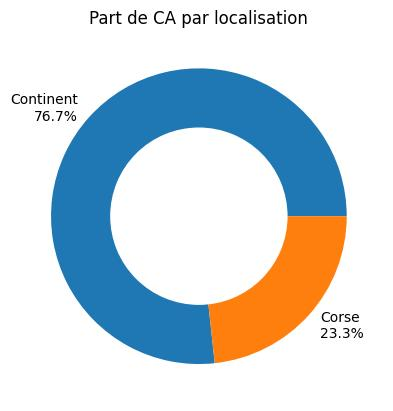
\includegraphics[width=1\textwidth]{assets/ca_par_localisation}
            \end{figure}
    \end{columns}

    {\hskip-3em\usebeamerfont{frametitle}\usebeamercolor[fg]{frametitle} Activité}

    \begin{columns}
        \column{0.33\textwidth}
            \centering

            \begin{figure}[h]
                \centering
                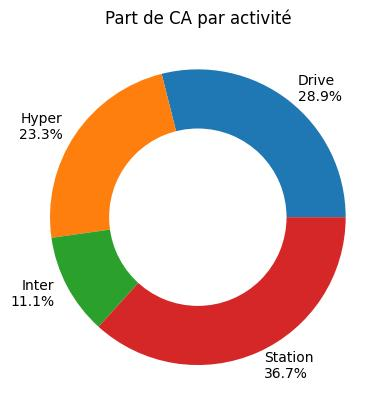
\includegraphics[width=1\textwidth]{assets/ca_par_activite}
            \end{figure}

        \column{0.66\textwidth}
            La visualisation ci-contre présente la répartition du CA par activité :

            \begin{itemize}
                <@ for activite, part_ca in ca_par_activite.items() @>
                    \item{Les points de vente \textbf{<< activite >>} représentent \textbf{<< part_ca|number(1) >>\%} du CA}
                <@ endfor @>
            \end{itemize}
    \end{columns}
\end{frame}
